% uofl-example.tex: an example how to use uofl.cls.
% $Id: uofl-example.tex,v 1.23 1997/07/22 16:30:27 tjchol01 Exp tjchol01 $

% The version of this file corresponds to the version of
% uofl.cls.  The text and additional formatting in this document
% obviously need a lot of work to be acceptable (even for an example :-).

\documentclass[MEng]{uofl}
% Available options (choose one from each line, asterisks show the defaults):
%   MEng, *MSc, PhD, PhDproposal -- to select the type of thesis/dissertation
%     (you can use command \target as a last resort for some strange thesis)
%   *EE, EMACS, CSE -- to select your department (\department{} works too)

% If you want to include C (CWEB) programs then you should uncomment
% the following line:
%\usepackage[nonumbers]{cwebprog}
\usepackage{libertine}
\usepackage{graphicx}
\graphicspath{ {../analysis/} }

\begin{document}

\title{Online Analysis of Disk I/O}
\author{Michael Thomas Marzullo}
\degree{B.S., University of Louisville, 2019}
\target{A Project\\
Submitted to the Faculty of the\\
University of Louisville\\
Speed Scientific School\\
as Partial Fulfillment of the Requirements\\
for the Professional Degree of}

%\department{Department of English\\
%University of Louisville\\
%Louisville, Kentucky}

\date{December 2019}
\department{Computer Science and Computer Engineering}
\committee{Dr. Nihat Altiparmak, Project Advisor}
\maketitle

\chapter*{ABSTRACT}
The move from hard disk drives to solid state drives has enabled a performance increase over an order of magnitude, 
and other state of the art technologies such as 3D XPoint have made another order of magnitude improvement over SSDs. 
These massive advancements in hardware have left gaps in the software which optimizes their usage so that their full 
potential can be utilized. We have developed a solution to identify correlations in block device writes in the Linux 
kernel in a real-time manner to improve the total I/O performance on high performance devices.

\chapter*{ACKNOWLEDGMENTS}
I would like to thank my advisor, Dr. Altiparmak, for his excellent guidance 
and instruction that have allowed the completion of this project. I would like to 
thank my family for always supporting me through my education and ensuring my 
success; my mother, Kristen, whom has always shown me the way when I have been 
lost, and my father, Peter, whom has inspired me to utilize my abilities to their
whole potential. Finally, I thank my friends for their support.

\blockofcontents

\chapter{Related Work}
For our analysis of disk I/O requests, we focus on collecting block correlations since they may be used to optimize parallel I/O performance, reduce the cost of Garbage Collection (GC), and improve general caching performance. To collect these correlations, frequent itemset mining (FIM) techniques can be used\cite{Li}. FIM algorithms take a series of transactions as input, and output associated items with a support value greater than a specified minimum.  Within the domain of FIM algorithms, there are offline and stream algorithms. An example of a basic offline FIM algorithm is the Apriori algorithm, which performs a scan of the transactions to first filter all items that are not frequent and then finds the associated items from the filtered input\cite{borge}. This algorithm has exponential computational complexity, making it inefficient for large itemsets. Another offline FIM algorithm, ECLAT (Equivalence Class Clustering and bottom-up Lattice Traversal), provides a large performance enhancement over the Apriori algorithm based on a depth-first search of intersecting transactions\cite{borge}. ECLAT can be executed in parallel and typically outperforms Apriori by an order of magnitude. One application of frequent itemset mining to the domain of block correlations has been explored by Li et al. in \textit{C-Miner: Mining Block Correlations in Storage Systems}\cite{Li}. C-Miner is an offline mining algorithm that can be used to find correlated blocks from sources such as file systems or databases. A “gap” measurement is defined to limit the maximum distance between frequent subsequences. This creates a sliding window in which C-Miner processes items, which limits the spatial locality. Temporal locality is not considered for the generated block association rules. Offline algorithms provide a basis for providing accurate correlation results, but they cannot be applied to perform optimizations in real-time for continuous data such as I/O streams.

Stream based FIM algorithms have been explored more recently to apply these data mining techniques to continuous data patterns, which are sourced from many domains in the real world (network traffic, GPS, sensor data). Shin et. al presented the estDec+ algorithm which implements a Compressible Prefix (CP) tree to dynamically accept items from a stream source \cite{Shin}. This tree structure adapts its performance to a configured memory size. The CP-tree merges and splits nodes to efficiently utilize the allocated memory space for the tree. The estDec+ algorithm’s accuracy is determined by the proportion of the allocated memory of the tree versus the size and throughput of the input stream.  However, the performance of streaming algorithms such as estDec+ is not applicable to extremely high throughput streams from high performance I/O devices. 

These stream algorithms also typically focus on generating the maximum frequent itemsets instead of frequently correlated pairs which we are attempting to find. The algorithm used for our goal must also must perform efficiently given a limited memory space and CPU resources to not reduce performance across the rest of the system. Instead of focusing on data mining through computationally expensive techniques, we focus on simpler methods used within computer architecture to achieve fast processing time and accurate results. Much research on caching methods has been performed for use with hardware and software. One example of a high-performance and influential cache structure, the Adaptive Replacement Cache (ARC) describes a cache that dynamically resizes based on access patterns \cite{Megiddo}. Optimal performance can be achieved without fixed user configuration of the cache size. The ARC consists of four separate LRU caches. The two main caches, T1 and T2, store recent items and frequent items (more than 1 hit) while the two other caches, B1 and B2, are ghost caches which store items that have been evicted. A fixed cache size is set for the two main caches, and the size of the two ghost caches is automatically tuned by the algorithm. In their experiments, ARC was shown to be superior to many other popular and well-known caching algorithms such as 2Q\cite{Megiddo}.


%\newpage\layout

\chapter{Implementation}

\section{Efficient Monitoring of Disk I/O}
The Linux blktrace utility is used to monitor all block layer I/O events. A user level and kernel level component is used to enable this functionality. The user-level blktrace accepts parameters such as the type of request to filter and the block device to monitor. When the utility is run, it signals the kernel component to enable monitoring. The output produced by the utility is in a binary format, so to convert them to a human-readable format, the blkparse utility is used to parse this output into a format specified by the user. This output can either be stored in a file or output to stdout. Because of this, the utility can only be used for offline analysis of block events. Along with this, the tool monitors all system activity and can only be filtered by the block device. Each event trace includes information such as the CPU id, command type, process id, time stamp, sector number, and offset. At the kernel level, an ioctl handler is used to receive the input from the user-level blktrace utility to both enable tracepoints within the block layer and set the parameters and filters requested by the user utility. The events are then communicated from the kernel to the user-level with a debugfs relay. 

To monitor storage I/O requests for specific applications, we developed a modification to the blktrace mechanism within the Linux kernel to filter traces sent to the user-level blktrace program by process id. 
In the kernel, the blk\_user\_trace\_setup struct was changed to include an additional integer array to store process identifiers to monitor. 
When this parameter is received by blktrace through the blk\_trace\_ioctl function, only I/O requests from the specified filter are forwarded to the userspace relay from the \_\_blk\_add\_trace function. 
The user blktrace utility was then modified to accept a pid parameter that may be set dynamically to monitor any applications needed. The binary output from blktrace is piped into blkparse, which acts as a writer to a named pipe containing the sector, offset, and timestamp of the request. This named pipe may then be read by another program to be used for online analysis. 

\section{Online Disk I/O Analysis Techniques}
We developed a multi-level caching algorithm that takes a data stream of transactions as input and processes them in real time to allow frequent block correlations to be queried by other systems. Multiple iterations of this algorithm were created to gradually improve performance and accuracy. The first iteration of the algorithm (implemented in Python) is described below. 

\subsection{Algorithm 1}
The basic architecture of the algorithm is a two-level cache with an additional eviction cache. The first level cache may act as either an LRU or LIFO cache with a configured maximum item count. This simple method is used as a first step in quickly filtering the large stream of items received. After an item count increases past a defined support threshold, the item is then inserted into the second level of the cache. This second level represents all frequent pairs and uses another hash table to store and retrieve the data. The items may then be evicted based on either a maximum sequence distance or time threshold. 

While the cache is running, a separate system generates a graph of all possible block associations to be queried by another application. The graph structure uses an adjacency matrix to store all block ids as individual vertices. This graph is created from the items in the L2 cache, then DFS is applied to output the connected components. Each connected component represents a grouping of block associations, and these are assigned a stream identifier to use through round-robin selection. 

When items are received by the algorithm from the named pipe, all possible block pairs are generated to be inserted in the L1 cache, which is an O($N^2$) operation. In our initial performance testing, this was found to be too slow to handle workloads such as large sequential writes in real time. Because of this lack of performance, more modifications were needed for a new algorithm.

\subsection{Algorithm 2}
In this modified algorithm, the received write operations from the tracing component are stored as intervals instead of generating all possible pairs. The primary data structure used to store these items is an interval tree, which is a modification of red-black tree that stores intervals in place of single values in the leaves of the tree. In addition, to further improve both the performance of the cache and the accuracy of the results to track both frequency and temporal locality, the first level cache structure from the first algorithm is replaced with the ARC algorithm previously described. This allows high performance throughput for I/O operations that contain a large range of blocks, while also handling and adapting overlapping operations on existing intervals within the red-black tree. The ARC also adapts its size to the input tree, which should decrease memory usage and increase accuracy. The advantage of using the combination of the ARC and interval tree is that items can be found in constant time while also processing I/O operations of any size in constant time. Once the support from the frequent LRU cache reaches the minimum threshold, the item is moved into the L2 frequent item cache, which is a combination of a LRU cache and interval tree. The eviction policy for the L2 cache is determined either by time passed or transactions processed. Since all of the operations within this algorithm are relatively computationally cheap (O($N$) for ARC, O($log N$) for the interval tree), this algorithm is able to handle the high throughput of system I/O in real time. 

Once the frequent itemsets are queried by another system, the algorithm generates the correlated block pairs from the L2 cache. The initial generation of the graph is not computationally cheap as the block correlations must be generated from all intervals present in the interval tree. The correlations are not updated constantly for this reason, and snapshots at specified intervals are used instead. This interval may be tuned based on how much drift there is within the workload. After the correlations are generated, they are stored in a hash table so that all queries will be completed with a low latency. 

\chapter{Experiments \& Methodology}
The experiments were run on a machine with an Intel Xeon E3-1230v5 with 64GB of RAM and a Samsung SM961 SSD. Fio was used as a synthetic benchmarking tool to demonstrate the performance and accuracy of our algorithm. Fio can generate workloads based on job configurations that may use a variety of different system interfaces and I/O request types. For our evaluation, we focused on creating workloads that contain blocks that are overwritten over defined sequences or times. This requires precise control of the sectors and block sizes written to the I/O device, and fio does not have any available configuration to produce these specific types of workloads. However, it does have functionality to replay the binary output from blktrace or the internal iolog format used by fio. To perform our experiments, we developed a tool to artificially create workloads in the form of the blktrace binary output, which is then replayed by fio. This tool allows us to define a distribution of sequential and random writes along with specific block ranges to repeatedly perform writes in a configured pattern. The synthetic workloads created were made to verify the algorithm’s correlation mining performance in three areas: spatial locality, temporal locality, and frequency. 

All workloads evaluated are performed on a 10GB block device, and no read operations are included in the traces. The drive has a 512B sector size, yielding 20971520 sectors. The workload generation tool creates writes using a uniform random distribution across the complete sector range along with a set of configured sectors with probabilities individually assigned. For these experiments, the effectiveness of the algorithm is evaluated through a simple accuracy metric: the fraction of blocks in the L2 cache that were configured to be randomly repeated in the workload. If the accuracy value is high, it demonstrates that the algorithm is able to mine randomly distributed patterns present in an I/O stream. The fixed size component $c$ is varied for the ARC along with the minimum support threshold to analyze how these parameters affect the performance of the algorithm. A bash script is used to perform the experiments in an automated manner, with blkparse, blktrace, fio, and the algorithm being started at the same time. For experiments where disk performance is measured, a TRIM command is performed on the whole block device to prevent garbage collection from impeding performance after multiple runs of the same experiment.

\begin{table}
    \caption{Experiments}
    \begin{center}
    \begin{tabular}{|c|c|c|c|c|} \hline
    Name&Size&Minimum Support&Sector Patterns&Pattern Probability \\ \hline
    Workload1 & 1m & 30 & 100 & 0.1\% \\ \hline
    Workload2 & 1m & 30 & 100 & 0.01\% \\ \hline
    Workload3 & 1m & 10 & 100 & 0.001\% \\ \hline
    Workload3ms5 & 1m & 5 & 100 & 0.001\% \\ \hline
    \end{tabular}
    \end{center}
    \label{tab:a}
\end{table}

\chapter{Results \& Discussion}
First, the the general I/O performance of tracing is recorded in Figure \ref{tracing}. This metric is crucial for the use of the algorithm as it should not significantly impede I/O operations as a whole, and the net gain provided by the optimizations should be greater than any decreases in overall throughput from mining the correlations. The graph displays the average bandwidth and IOPS over 3 runs of a 4K Random Write trace. It is observed that there was a minor decrease for both bandwidth and IOPS, but this is not enough to be severely concerned about the tracing mechanisms performance. 

The experiments used to evaluate accuracy are described in Table 1. For each workload, a different synthetic trace is used with the parameters specified. The pattern probability is varied to observe the algorithm performance with different granularities of writes. The minimum support is adjusted for these workloads in accordance with the probabilities set, as the expected number of patterns appearing in the trace change. It is expected that the algorithm produces output of only the patterns configured in the trace, and not the random noise of the other writes in the L2 frequent item cache when the trace completes. The results of the experiments were consistent with our expectations, and the accuracy for each workload was graphed across a number of different main cache sizes. Figures \ref{w1}-\ref{w3ms5} display the results for each experiment. For Workload1 and Workload2, the pattern probabilities were high enough that the algorithm achieved 100\% accuracy for all cache sizes. Workload3 provided a challenge for the algorithm, as it had a maximum 37\% accuracy with the largest cache size tested of 250k items. Decreasing the minimum support to 5 increased the maximum accuracy to 91\% for the same trace without outputting any irrelevant patterns. It is observed that in all cases, increasing the ARC cache size only marginally increases the accuracy of patterns detected. This shows that the ARC is not heavily dependent on the size of the main cache size, and it appropriately adapts the ghost cache size based on the input stream. The results from these experiments demonstrate that the developed tracing mechanism and algorithm are viable for detecting patterns that are both relatively frequent and infrequent in an input stream. 

\chapter{Conclusions}
The results in this project provide multiple contributions: 
\begin{enumerate}
    \item A high performance, process specific I/O monitoring patch for the Linux kernel
    \item A tool for producing synthetic I/O traces that contain configurable patterns to be used with either fio or blkreplay 
    \item An advanced caching algorithm for mining frequent block correlations from a \\ stream of system I/O requests
\end{enumerate}

These contributions allow experimentation and online analysis of disk I/O, which can then be used for optimization of storage systems through both hardware and software. Optimization in hardware can be accomplished through open-channel SSDs to maximize internal parallelism, and to also organize data to minimize garbage collection. In software, application-specific caching can be performed to increase performance. 

The research and work completed span many domains in computer science. Data mining techniques were extensively reviewed and tested to find approaches applicable to the goal of finding block correlations from a stream. Understanding of the Linux kernel and systems level programming was also necessary to develop the tracing mechanism. The algorithm itself required research of many advanced data structures and computer architecture to determine a solution that was both efficient and accurate.

\chapter{Future Work}
Due to time limitations, many experiments relevant to this project were not completed. In the future, we plan to use many other techniques that can fully utilize all of our tools to identify any weaknesses and areas of improvement. The only distribution tested in our synthetic workload experiments was the random uniform distribution, which may not always represent real workloads present on a machine. This could be supplemented by performing similar experiments with different distributions of the repeated patterns such as the Zipf distribution. In addition to our synthetic workloads, it is necessary to also experiment with traces from real applications. These experiments could be created either through replaying traces through fio for different workload types (web, database, fileserver) or through using our monitoring tools directly on a running application. In addition to the analysis of FIM performance, experiments for the possible optimizations at the hardware level can be created. Our main goal in this project was to reduce garbage collection costs within SSDs, but this cannot be tested in real hardware at this time since open-channel SSDs are not commercially available. Instead, a simulator of an open-channel SSD can be used so that the stream output of our algorithm can be evaluated. System performance metrics have also not been formally reported. We have developed an algorithm that can handle the throughput of an I/O stream, but the total CPU and memory usage needs to be compared to the tunable parameters. 

For the algorithm itself, there are still some obvious optimizations that have not been completed. Python was chosen as the current implementation language for increased productivity while determining a successful architecture, but our final architecture will be converted to a lower level systems programming language such as C++ so that the system resources needed to run the algorithm can be reduced significantly. The architecture can also be improved through automatic parameter tuning. Although the ARC already dynamically sizes the ghost caches based on the input data stream, the main caches use a fixed size. New eviction policies may also be needed for the L2 cache after experimentation is completed for real-world workloads. 

In the tracing mechanism, one weakness in the current implementation is that these modifications cannot filter block level operations that are created through asynchronous I/O system calls. When these I/O operations are performed, the process id passed to the block layer from the kernel is zero instead of the original process id, which means that they cannot be appropriately identified and therefore cannot be filtered. An additional modification in the kernel is required to either pass the original process id to the block layer or track the requests in another manner entirely. 

\appendix
\chapter{Figures}
\begin{figure}
    \caption{Tracing Flowchart}
    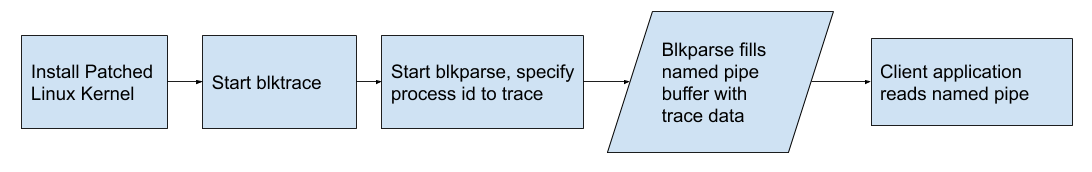
\includegraphics[width=\columnwidth]{d1.png}
    \label{tracingf}
\end{figure}

\begin{figure}
    \caption{Algorithm 1 Flowchart}
    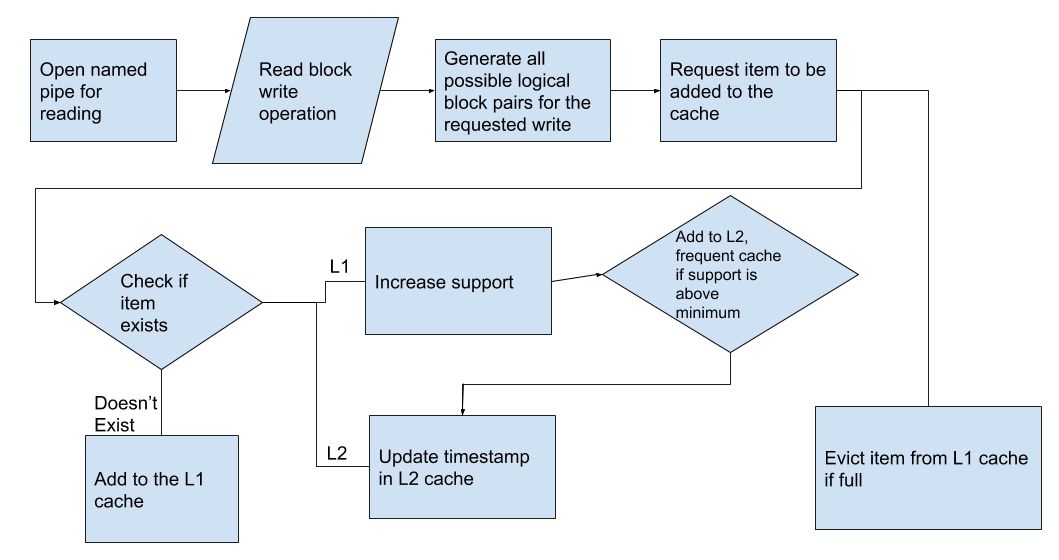
\includegraphics[width=\columnwidth]{d2.png}
    \label{a1}
\end{figure}

\begin{figure}
    \caption{Algorithm 2 Flowchart}
    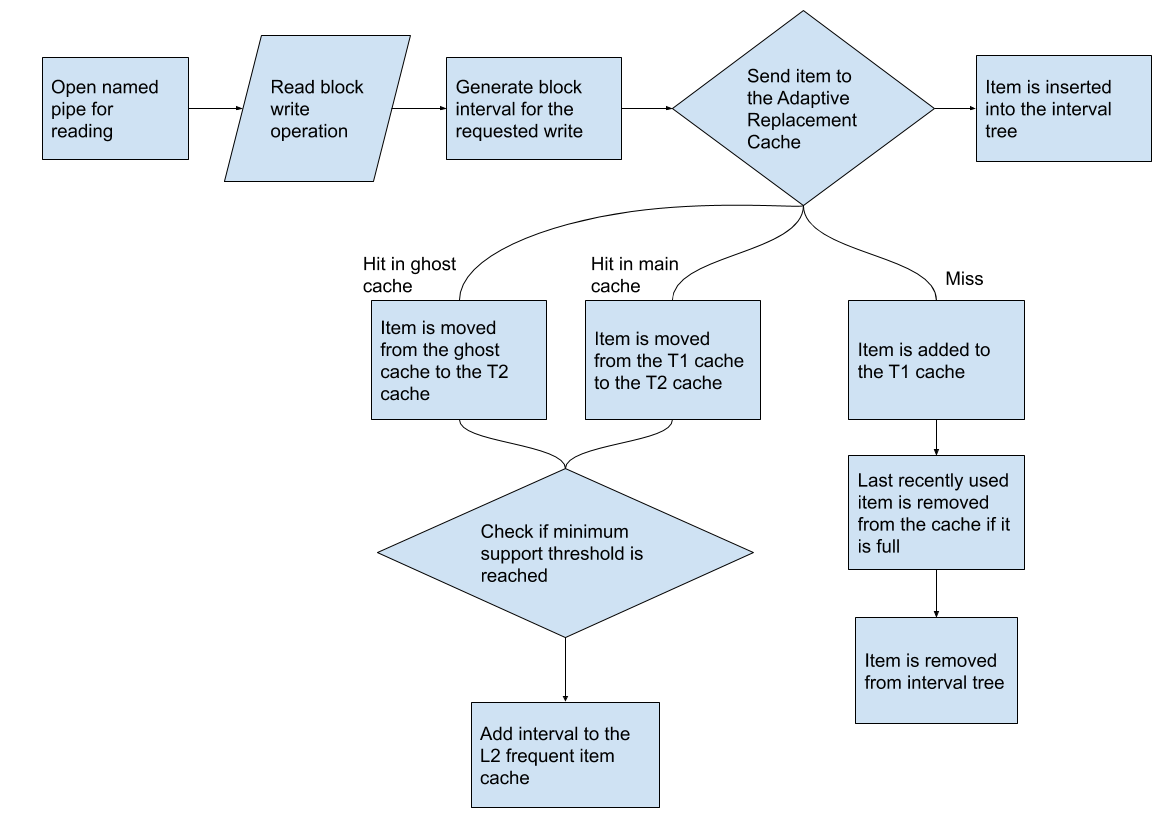
\includegraphics[width=\columnwidth]{d3.png}
    \label{a2}
\end{figure}

\begin{figure}
    \caption{Stream Generation Flowchart}
    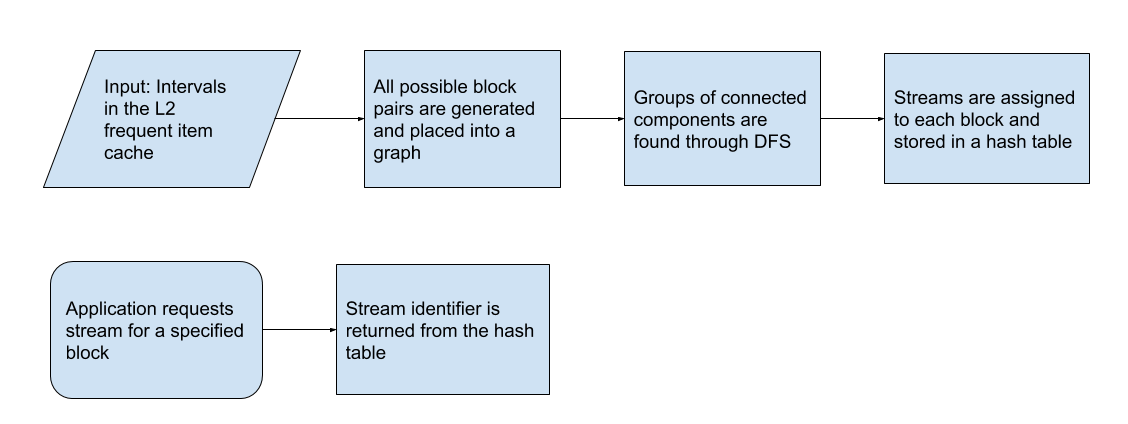
\includegraphics[width=\columnwidth]{d4.png}
    \label{sg}
\end{figure}

\begin{figure}
    \caption{Tracing Performance}
    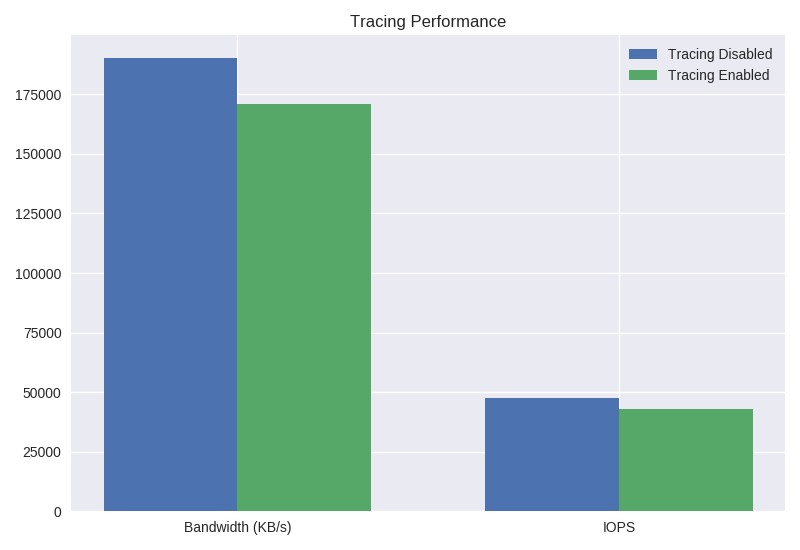
\includegraphics[width=\columnwidth]{bandwidth1.png}
    \label{tracing}
\end{figure}

\begin{figure}
    \caption{Workload1 Accuracy}
    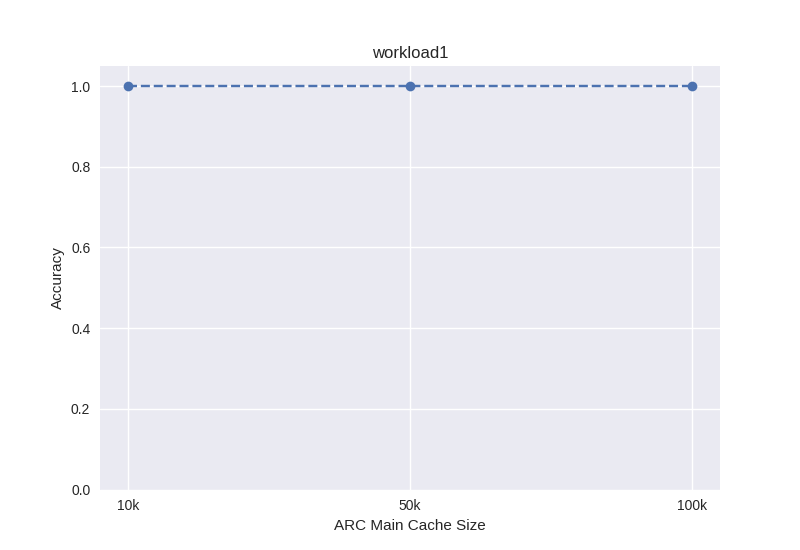
\includegraphics[width=\columnwidth]{workload1.png}
    \label{w1}
\end{figure}

\begin{figure}
    \caption{Workload2 Accuracy}
    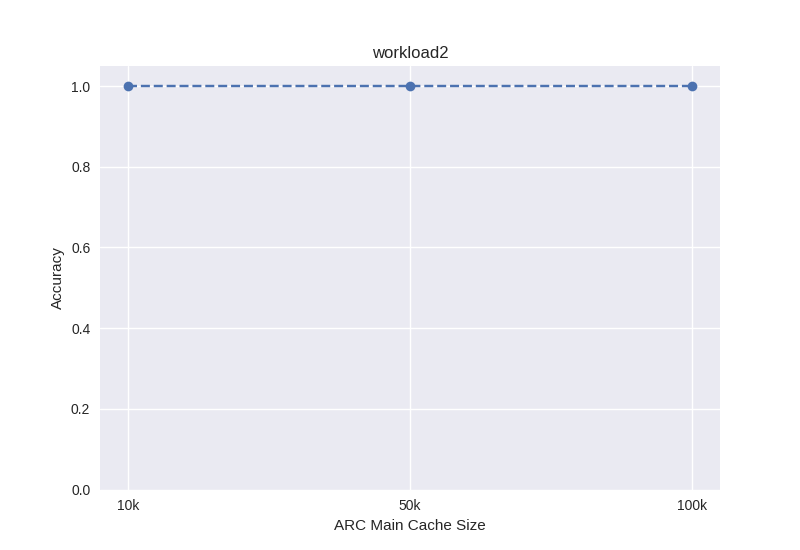
\includegraphics[width=\columnwidth]{workload2.png}
    \label{w2}
\end{figure}

\begin{figure}
    \caption{Workload3 Accuracy}
    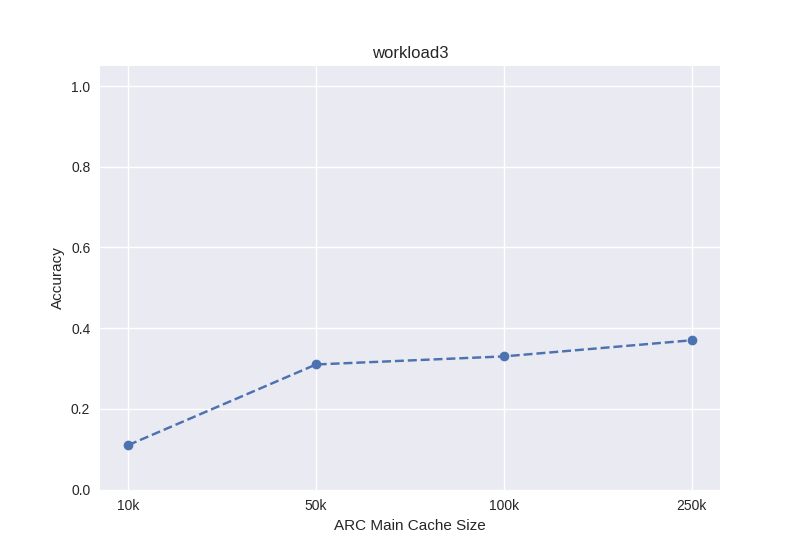
\includegraphics[width=\columnwidth]{workload3.png}
    \label{w3}
\end{figure}

\begin{figure}
    \caption{Workload3ms5 Accuracy}
    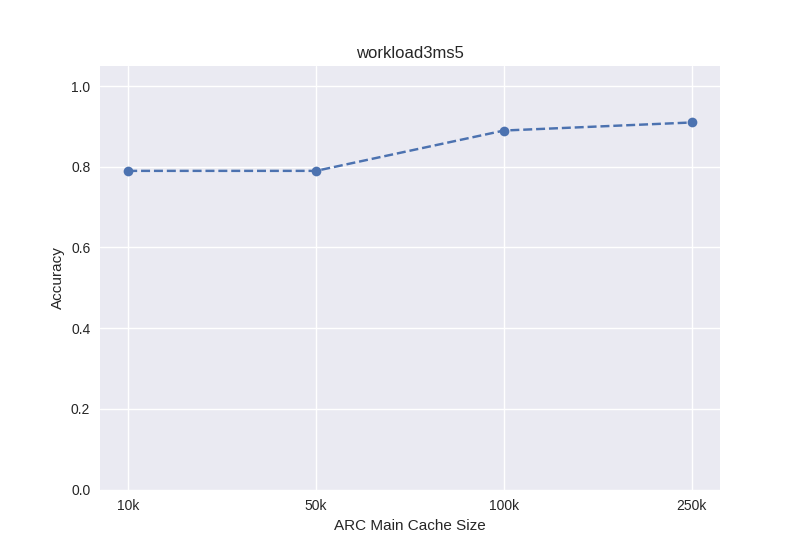
\includegraphics[width=\columnwidth]{workload3ms5.png}
    \label{w3ms5}
\end{figure}

\chapter{Source Code}

The source code for this project can be found at https://github.com/UOFL-CSL.

\bibliographystyle{unsrt}

\nocite{vStream}
\nocite{streampc}
\nocite{ladaptivereplace}
\bibliography{references.bib}


\end{document}
